	\documentclass[a4paper, 12pt]{article} % тип документа

%%%Библиотеки
	%\usepackage[warn]{mathtext}	
	\usepackage[T2A]{fontenc}   %Кодировка
	\usepackage[utf8]{inputenc} %Кодировка исходного текста
	\usepackage[english, russian]{babel} %Локализация и переносы
	\usepackage{caption}
	\usepackage{listings}
	\usepackage{amsmath, amsfonts, amssymb, amsthm, mathtools}
	\usepackage[warn]{mathtext}
	\usepackage[mathscr]{eucal}
	\usepackage{wasysym}
	\usepackage{graphicx} %Вставка картинок правильная
	\DeclareGraphicsExtensions{.pdf,.png,.jpg}
	\graphicspath{ {images/} }
	
	\setlength{\parskip}{0.5cm}
	
	\usepackage{pgfplots}
	\usepackage{indentfirst}
	\usepackage{float}    %Плавающие картинки
	\usepackage{wrapfig}  %Обтекание фигур (таблиц, картинок и прочего)
	\usepackage{fancyhdr} %Загрузим пакет
	\usepackage{lscape}
	\usepackage{xcolor}
	\usepackage[normalem]{ulem}
	\usepackage{wasysym}
	
	\usepackage{titlesec}
	\titlelabel{\thetitle.\quad}

	\usepackage{hyperref}
	\newenvironment{comment}{}{}

%%%Конец библиотек

%%%Настройка ссылок
	\hypersetup
	{
		colorlinks = true,
		linkcolor  = blue,
		filecolor  = magenta,
		urlcolor   = blue
	}
%%%Конец настройки ссылок


%%%Настройка колонтитулы
	\pagestyle{fancy}
	\fancyhead{}
	\fancyhead[L]{2.4.1}
	\fancyhead[R]{Старченко Иван, группа Б01-005}
	\fancyfoot[C]{\thepage}
%%%конец настройки колонтитулы

\begin{document}

\setcounter{page}{1}



\begin{center}
  \LARGE{Лабораторная работа 2.1.6}\\[0.2cm]
  \LARGE{Эффекта Джоуля-Томсона.}\\[0.2cm]
  \large{24 февраля 2021 г.}\\[0.2cm]
  \large{Старченко Иван Александрович}\\[0.2cm]
\end{center}

\textbf{Цель работы:} \\
1) Определение изменения температуры углекислого газа при проте-кании через малопроницаемую перегородку при разных начальных значениях давления и температуры.\\
2) Вычисление по результатам опытов коэффициентов Ван-дер-Ваальса $a$ и $b$.

\textbf{В работе используются:} \\
Трубка с пористой перегородкой, труба Дьюара, термостат, термометры, дифференциальная термопара, микровольтметр, балластный баллон, манометр.


\begin{center}
	\large{\textbf{Теоретические сведения}}
\end{center}

Эффектом Джоуля–Томсона называется изменение температуры газа, медленно протекающего из области высокого в область низкого давления в условиях хорошей тепловой изоляции. В разреженных газах, которые приближаются по своим свойствам к идеальному газу, при таком течении температура газа не меняется. Эффект Джоуля–Томсона демонстрирует отличие исследуемого газа от идеального.\\

\begin{figure}[h!]
\centering{
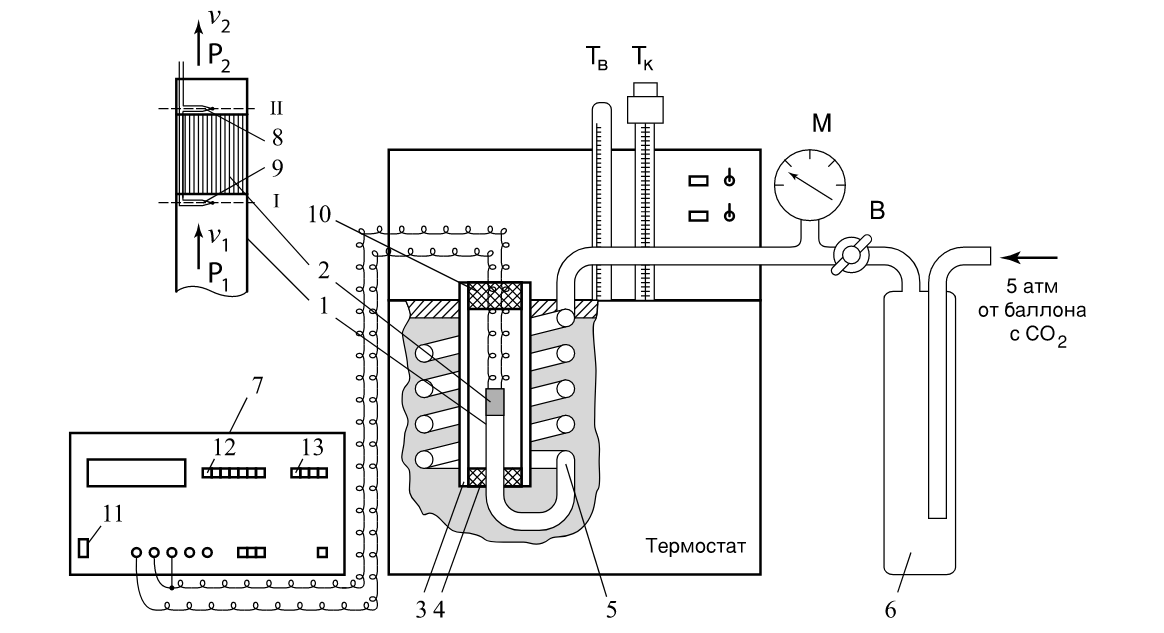
\includegraphics[width=15cm]{scheme.png}
}
\caption{Схема установки для изучения эффекта Джоуля–Томсона.}
\end{figure}

В работе исследуется изменение температуры углекислого газа при медленном его течении по трубке с пористой перегородкой (рис. 1). Трубка 1 хорошо теплоизолирована. Газ из области повышенного давления $P_1$ проходит через множество узких и длинных каналов пористой перегородки 2 в область с атмосферным давлением $P_2$. Перепад давления $\Delta P = P_1 - P_2$ из-за большого сопротивления каналов может быть заметным даже при малой скорости течения газа в трубке. Величина эффекта Джоуля–Томсона определяется по разности температуры газа до и после перегородки.\\

Рассмотрим стационарный поток газа между произвольными сечениями I и II трубки (до перегородки и после нее). Пусть, для определенности, через трубку прошел 1 моль углекислого газа; $\mu$ --- его молярная масса. Молярные объемы газа, его давления и отнесенные к молю внутренние энергии газа в сечениях I и II обозначим соответственно $V_1, P_1, U_1$ и $V_2, P_2, U_2$. Для того чтобы ввести в трубку объем $V_1$, над газом нужно совершить работу $A_1 = P_1V_1$. Проходя через сечение II, газ сам совершает работу $A_2 = P_2V_2$. Так как через боковые стенки не происходит ни обмена теплом, ни передачи механической энергии, то:

\begin{equation}
A_1 - A_2 = \left(U_2 + \dfrac{\mu v_2^2}{2}\right) - \left(U_1 + \dfrac{\mu v_1^2}{2}\right).
\end{equation}

В уравнении (1) учтено изменение как внутренней (первые члены в скобках), так и кинетической (вторые члены в скобках) энергии газа. Подставляя в (1) написанные выражения для $A_1$ и $A_2$ и перегрупп ровывая члены, найдем:

\begin{equation}
H_1 - H_2 = (U_1 + P_1V_1) - (U_2 + P_2V_2) = \dfrac{1}{2} \mu (v_2^2 - v_1^2).
\end{equation}

Сделаем несколько замечаний. Прежде всего отметим, что в процессе Джоуля–Томсона газ испытывает в пористой перегородке суще- ственное трение, приводящее к ее нагреву. Потери энергии на нагрев трубки в начале процесса могут быть очень существенными и сильно искажают ход явления. После того как температура трубки установится и газ станет уносить с собой все выделенное им в пробке тепло, формула (1) становится точной, если, конечно, теплоизоляция трубки достаточно хороша и не происходит утечек тепла наружу через ее стенки.\\

Второе замечание связано с правой частью (2). Процесс Джоуля–Томсона в чистом виде осуществляется лишь в том случае, если правой частью можно пренебречь, т.~е. если макроскопическая скорость газа с обеих сторон трубки достаточно мала. У нас сейчас нет критерия, который позволил бы установить, когда это можно сделать. Поэтому мы отложим на некоторое время обсуждение вопроса о правой части (2), а пока будем считать, что энтальпия газа не меняется.

\begin{equation}
\mu_{Д-Т} = \dfrac{\Delta T}{\Delta P} \approx \dfrac{\frac{2a}{RT}-b}{C_p}.
\end{equation}

Отсюда видно, что эффект Джоуля–Томсона для не очень плотного газа зависит от соотношения величин $a$ и $b$, которые оказывают противоположное влияние на знак эффекта. Если силы взаимодействия между молекулами велики, так что превалирует <<поправка на давление>>, то основную роль играет член, содержащий $a$, и

\begin{equation}
\dfrac{\Delta T}{\Delta P} > 0,
\end{equation}

то есть газ при расширении охлаждается ($\Delta T < 0$, так как всегда $\Delta P < 0$). В обратном случае (малые $a$)

\begin{equation}
\dfrac{\Delta T}{\Delta P} < 0,
\end{equation}

то есть газ нагревается ($\Delta T > 0$, так как по-прежнему $\Delta P < 0$).\\

Этот результат нетрудно понять из энергетических соображений. Как мы уже знаем, у идеального газа эффект Джоуля–Томсона отсутствует. Идеальный газ отличается от реального тем, что в нем можно пренебречь потенциальной энергией взаимодействия молекул. Наличие этой энергии приводит к охлаждению или нагреванию реальных газов при расширении. При больших $a$ велика энергия притяжения молекул. Это означает, что потенциальная энергия молекул при их сближении уменьшается, а при удалении --- при расширении газа --- возрастает. Возрастание потенциальной энергии молекул происходит за счет их кинетической энергии --- температура газа при расширении падает. Аналогичные рассуждения позволяют понять, почему расширяющийся газ нагревается при больших значениях $b$.\\

Как следует из формул (1.35), (1.36), при температуре $T_i$ коэффициент $\mu_{Д-Т} $ обращается в нуль. Используя связь между коэффициентами $a$ и $b$ и критической температурой (1.19), по формуле (1.36) найдем

\begin{equation}
T_{инв} = \dfrac{27}{4}T_{кр}.
\end{equation}


При температуре $T_{инв}$ эффект Джоуля–Томсона меняет знак: ниже температуры инверсии эффект положителен ($\mu_{Д-Т} > 0$, газ охлаждается), выше $T_{инв}$ эффект отрицателен ($\mu_{Д-Т} < 0$, газ нагревается).\\

Температура инверсии у всех газов лежит значительно выше критической. Для большинства газов $T_{инв}/T_{кр} = 5-8$. Например, для гелия $T_{инв} = 46К, T_{кр} = 5,2К$; для водорода $T_{инв} = 205К, T_{кр }= 33К;$ для азота $T_{инв} = 604 К, T_{кр} = 126 К;$ для воздуха $T_{инв} = 650 К, T_{кр} = 132,6 К$; для углекислого газа $T_{инв} = 2050 К, T_{кр} = 304 К.$ Температура инверсии у гелия и водорода значительно ниже комнатной, поэтому при обычных температурах эти газы при расширении нагреваются. Температура инверсии остальных газов выше комнатной, и при нормальных условиях температура при расширении газа падает.\\

Сравнивая приведенные значения $T_{инв}$ и $T_{кр}$, можно убедиться в том, что предсказания, следующие из формулы Ван-дер-Ваальса, у реальных газов выполняются не очень хорошо. Правильно передавая качественную картину поведения реальных газов, формула Ван-дер-Ваальса не претендует на хорошее количественное описание этой картины.\\

При больших изменениях давления, например, при дросселировании от 200 до 1 атм (интегральный эффект Джоуля–Томсона), как это нередко бывает в промышленных установках, разложением (1.28) пользоваться нельзя и приходится прибегать к общему соотношению (1.26). При этом связь между температурой и давлением находится с помощью специальных диаграмм, например, кривых $H = const$, проведенных в координатах температура-давление или температура-энтропия. Такие диаграммы строятся по экспериментальным данным и широко используются в технике.\\

Вернемся к влиянию правой части уравнения (2) на изменение температуры расширяющегося газа. Для этого сравним изменение температуры, происходящее вследствие эффекта Джоуля–Томсона, с
изменением температуры, возникающим из-за изменения кинетической энергии газа . Увеличение кинетической энергии газа вызывает заметное и приблизительно одинаковое понижение его температуры как у реальных, так и у идеальных газов. Поэтому при оценках нет смысла пользоваться сложными формулами для газа Ван-дер-Ваальса.\\

Заменяя в формуле (2) $U$ через $C_V T$ и $P V$ через $RT$, найдем

\begin{equation}
(R+C_V)(T_1 - T_2) = \mu(v_2^2 - v_1^2)/2,
\end{equation}

или

\begin{equation}
\Delta T = \dfrac{\mu}{2C_p} (v_2^2 - v_1^2).
\end{equation}

В условиях нашего опыта расход газа $Q$ на выходе из пористой перегородки не превышает 10 $см^3/с$, а диаметр трубки равен 3 мм. Поэтому

\begin{equation}
v_2\cdot \dfrac{4Q}{\pi d^2} \approx 140 см/с.
\end{equation}

Скорость $v_1$ газа у входа в пробку относится к скорости $v_2$ у выхода из нее как давление $P_2$ относится к $P_1$. В нашей установке $P_1$ = 4 атм, a $P_2$ = 1 атм, поэтому

\begin{equation}
v_1 = \dfrac{P_2}{P_1} v_2 = 35 см/с.
\end{equation}

Для углекислого газа $\mu$ = 44 г/моль, $C_p$ = 40 Дж/($моль \cdot К$); имеем

\begin{equation}
\Delta T = \dfrac{\mu}{2C_p} (v_2^2 - v_1^2) = 7 \cdot 10^{-4} К.
\end{equation}

Это изменение температуры ничтожно мало по сравнению с измеряемым эффектом (несколько градусов).\\

В данной лабораторной работе исследуется коэффициент дифференциального эффекта Джоуля–Томсона для углекислого газа. По экспериментальным результатам оценивается коэффициент теплового расширения, постоянные в уравнении Ван-дер-Ваальса и температура инверсии углекислого газа. Начальная температура газа $T_1$ задается термостатом. Измерения проводятся при трех температурах: комнатной, $50\degree С$ и $80 \degree С$.

\textbf{Экспериментальная установка.}
Схема установки для исследования эффекта Джоуля–Томсона в углекислом газе см. рис. 1. Основным элементом установки является трубка 1 с пористой перегородкой 2, через которую пропускается исследуемый газ. Трубка имеет длину 80 мм и сделана из нержавеющей стали, обладающей, как известно, малой теплопроводностью. Диаметр трубки $d = 3$ мм, толщина стенок $0,2$ мм. Пористая перегородка расположена в конце трубки и представляет собой стеклянную пористую пробку со мно- жеством узких и длинных каналов. Пористость и толщина пробки ($l = 5$ мм) подобраны так, чтобы обеспечить оптимальный поток газа при перепаде давлений $\Delta P \approx$ 4 атм (расход газа составляет около 10 $см^3/с$); при этом в результате эффекта Джоуля–Томсона создается достаточная разность температур.\\

Углекислый газ под повышенным давлением поступает в трубку через змеевик 5 из балластного баллона 6. Медный змеевик омывается водой и нагревает медленно протекающий через него газ до температуры воды в термостате. Температура воды измеряется термометром $T_в$, помещенным в термостате. Требуемая температура воды устанавливается и поддерживается во время эксперимента при помощи контактного термометра $Tк$.

Давление газа в трубке измеряется манометром М и регулируется вентилем В (при открывании вентиля В, то есть  при повороте ручки против часовой стрелки, давление $P_1$ повышается). Манометр М измеряет разность между давлением внутри трубки и наружным (атмосферным) давлением. Так как углекислый газ после пористой перегородки выходит в область с атмосферным давлением $P_2$, то этот манометр непосредственно измеряет перепад давления на входе и на выходе трубки $\Delta P = P1 - P2.$\\

Разность температур газа до перегородки и после нее измеряется дифференциальной термопарой медь-константан. Константановая проволока диаметром 0,1 мм соединяет спаи 8 и 9, а медные проволоки (того же диаметра) подсоединены к цифровому вольтметру 7. Отвод тепла через проволоку столь малого сечения пренебрежимо мал. Для уменьшения теплоотвода трубка с пористой перегородкой помещена в трубу Дьюара 3, стенки которой посеребрены, для уменьшения теплоотдачи, связанной с излучением. Для уменьшения теплоотдачи за счет конвекции один конец трубы Дьюара уплотнен кольцом 4, а другой закрыт пробкой 10 из пенопласта. Такая пробка практически не создает перепада давлений между внутренней полостью трубы и атмосферой.\\
\begin{center}
	\large{\textbf{Обработка данных}}
\end{center}

Проведем изменения параметров для трёх различных значений температуры: $Т_1 =20\degree\ C$, $Т_2 = 30\degree\ C$, $Т_3 = 50\degree\ C$. Результат измерения перепада давления,  напряжения на термопаре и рассчитанную по формуле $\Delta T = \displaystyle\frac{E}{K}$ (с учетом $\Delta U(0)$) занесем в \textit{Таблицу 1}. 



\begin{center}
\begin{tabular}{ccc}
	$Т_1 =20$ & $Т_2 = 30$ & $Т_3 = 50$\\
	\begin{tabular}{|c|c|c|} \hline
		$p,\,\text{бар}$ & $V,\,\text{мВ}$ & $\Delta T_1, \degree\ C$ \\ \hline
		$4.0$ & $134.0$ & $3.37$\\ \hline 
		$3.5$ & $120.0$ & $3.02$\\ \hline 
		$3.0$ & $98.0 $ & $2.46$\\ \hline 
		$2.5$ & $76.0 $ & $1.90$\\ \hline 
		$2.0$ & $57.0 $ & $1.43$\\ \hline 
	\end{tabular}&
	\begin{tabular}{|c|c|c|} \hline
		$p,\,\text{бар}$ & $V,\,\text{мВ}$ & $\Delta T_2, \degree\ C$\\ \hline
		$4.0$ & $130.0$ & $3.02$\\ \hline 
		$3.5$ & $112.0$ & $2.75$\\ \hline 
		$3.0$ & $93.0 $ & $2.29$\\ \hline 
		$2.5$ & $74.0 $ & $1.82$\\ \hline 
		$2.0$ & $54.0 $ & $1.33$\\ \hline 
	\end{tabular}&
	\begin{tabular}{|c|c|c|} \hline
		$p,\,\text{бар}$ & $V,\,\text{мВ}$ & $\Delta T_3, \degree\ C$\\ \hline
		$4.0$ & $115.0$ & $2.71$\\ \hline 
		$3.5$ & $101.0$ & $2.38$\\ \hline 
		$3.0$ & $81.0 $ & $1.91$\\ \hline 
		$2.5$ & $66.0 $ & $1.55$\\ \hline 
		$2.0$ & $53.0 $ & $1.25$\\ \hline  
		\end{tabular}\\ \\
\end{tabular}
\textit{Таблица 1}
\end{center}

Из построенного графика зависимости $\Delta T$ от $\Delta P$ в Matlab, приведенного в конце работы, получим коэффициент наклона для каждой из температур и оценим их погрешность:
\[\mu_{D-T_1} = 0.99\cdot 10^{-5}\ \frac{К}{Па},\]
\[\mu_{D-T_2} = 0.93\cdot 10^{-5}\ \frac{К}{Па},\]
\[\mu_{D-T_3} = 0.75\cdot 10^{-5}\ \frac{К}{Па},\]

Систематическая погрешность будет состоять из погрешности манометра равная 		$\sigma_{\Delta p} = 0.1 бар$, погрешность вольтметра можно пренебречь по сравнению с погрешностью манометра.

Найдем погрешность аппроксимации по методу МНК:
\[\sigma_{\mu} = \sqrt{\frac{1}{n-1}\cdot \bigg(\frac{<\Delta T^2> - <\Delta T>^2}{<\Delta P^2> - <\Delta P>^2} - \mu^2\bigg)}\]
\[\sigma_{\mu_{D-T_1}} = 0.03\cdot 10^{-5}\ \frac{К}{Па},\]
\[\mu_{D-T_1} = (0.99 \pm 0.03)\cdot 10^{-5}\ \frac{К}{Па},\]
\[\sigma_{\mu_{D-T_2}} = 0.01\cdot 10^{-5}\ \frac{К}{Па},\]
\[\mu_{D-T_2} = (0.93 \pm 0.01)\cdot 10^{-5}\ \frac{К}{Па},\]
\[\sigma_{\mu_{D-T_3}} = 0.02\cdot 10^{-5}\ \frac{К}{Па},\]
\[\mu_{D-T_3} = (0.74 \pm 0.02)\cdot 10^{-5}\ \frac{К}{Па},\]

Найдем относительную погрешность $\mu$:
\[\varepsilon_{\mu} = \frac{\sigma_{\mu}}{\mu}\cdot 100\%\]
\[\varepsilon_{\mu_{D-T_1}} = 3.0\%\]
\[\varepsilon_{\mu_{D-T_2}} = 1.1\%\]
\[\varepsilon_{\mu_{D-T_3}} = 2.7\%\]

Воспльзуемся формулой $\mu_{Д-Т} = \dfrac{\Delta T}{\Delta P} \approx \dfrac{\frac{2a}{RT}-b}{C_p}$ и определим значения коэффициентов в уравнении Ван-дер-Ваальса. Также по формуле $Т_{инв} = \dfrac{2a}{Rb}$ определим температуру инверсии. Получим:
\[a = \frac{R\cdot C_p}{2}\cdot \frac{\mu_1 - \mu_2}{\frac{1}{T_1} - \frac{1}{T_2}}\]
\[b = C_p\cdot \frac{\mu_2\cdot T_2 - \mu_1\cdot T_1}{T_2 - T_1}\]

Между температурой $T_1 = 20\degree\ C$ и $T_2 = 30 \degree\ C$:
\[a_{20-30} = 0.90\ \frac{Па\cdot м^6}{моль^2},\]
\[b_{20-30} = 3.40\cdot 10^{-4} \frac{м^3}{моль},\]
\[a_{30-50} = 1.50\ \frac{Па\cdot м^6}{моль^2},\]
\[b_{30-50} = 8.11\cdot 10^{-4} \frac{м^3}{моль},\]

Найдем температуру инверсии:
\[T_{инв_1} = 636.79 К,\]
\[T_{инв_2} = 442.69 К,\]

Рассчитаем погрешности по формулам:
\[\sigma_{a} = a\cdot \bigg(\frac{\sigma_{\mu_1}}{\mu_1} + \frac{\sigma_{\mu_2} }{\mu_2}\bigg)\]
\[\sigma_{b} = b\cdot \bigg(\frac{\sigma_{\mu_1}}{\mu_1} + \frac{\sigma_{\mu_2} }{\mu_2}\bigg)\]
\[\sigma_{T_{инв}} 
= T_{инв}\cdot \sqrt{\bigg(\frac{\sigma_{a}}{a}\bigg)^2 + \bigg(\frac{\sigma_{b}}{b}\bigg)^2}\]

Получаем:
\[\sigma_{a_{20-30}} = 0.04\ \frac{Па\cdotм^6}{моль^2}\]
\[\sigma_{b_{20-30}} = 0.14\cdot 10^{-4} \frac{м^3}{моль}\]
\[\sigma_{a_{30-50}} = 0.06\ \frac{Па\cdot м^6}{моль^2}\]
\[\sigma_{b_{30-50}} = 0.33\cdot 10^{-4} \frac{м^3}{моль}\]
\[\sigma_{T_{инв_1}} = 65.5 К,\]
\[\sigma_{T_{инв_2}} = 35.59 К,\]

В итоге:
\[a_{20-30}  = (0.90\pm 0.04)\ \frac{Па\cdot м^6}{моль^2},\]
\[b_{20-30}  = (3.40\pm 0.14)\cdot 10^{-4} \frac{м^3}{моль},\]
\[a_{30-50} = (1.50\pm 0.06)\ \frac{Па\cdot м^6}{моль^2},\]
\[b_{30-50}  = (8.11\pm 0.33)\cdot 10^{-4} \frac{м^3}{моль},\]
\[T_{инв_1} = (636.79\pm 65.5)\ К,\]
\[T_{инв_2} = (442.69\pm 35.59)\ К,\]

Найдем относительную погрешность:
\[\varepsilon_{a_{20-30}} = 4.4\%\]
\[\varepsilon_{b_{20-30}} = 4.1\%\]
\[\varepsilon_{a_{30-50}} = 4.0\%\]
\[\varepsilon_{b_{30-50}} = 4.0\%\]
\[\varepsilon_{T_{инв_1}} = 10.2\%\]
\[\varepsilon_{T_{инв_2}} = 8.0\%\]

\begin{center}
	\large{\textbf{Вывод}}
\end{center}

В данной работе был изучен эффект Джоуля-Томсона. Найдены коэффциенты Джоуля-Томсона:
\[\mu_{D-T_1} = (0.99 \pm 0.03)\cdot 10^{-5}\ \frac{К}{Па},\]
\[\varepsilon_{\mu_{D-T_1}} = 3.0\%\]
\[\mu_{D-T_2} = (0.93 \pm 0.01)\cdot 10^{-5}\ \frac{К}{Па},\]
\[\varepsilon_{\mu_{D-T_2}} = 1.1\%\]
\[\mu_{D-T_3} = (0.74 \pm 0.02)\cdot 10^{-5}\ \frac{К}{Па},\]
\[\varepsilon_{\mu_{D-T_3}} = 2.7\%\]

Полученны коэффициентв Джоуля-Томсона:
\[a_{20-30}  = (0.90\pm 0.04)\ \frac{Па\cdot м^6}{моль^2},\]
\[\varepsilon_{a_{20-30}} = 4.4\%\]
\[b_{20-30}  = (3.40\pm 0.14)\cdot 10^{-4} \frac{м^3}{моль},\]
\[\varepsilon_{b_{20-30}} = 4.1\%\]
\\
\[a_{30-50} = (1.50\pm 0.06)\ \frac{Па\cdot м^6}{моль^2},\]
\[\varepsilon_{a_{30-50}} = 4.0\%\]
\[b_{30-50}  = (8.11\pm 0.33)\cdot 10^{-4} \frac{м^3}{моль},\]
\[\varepsilon_{b_{30-50}} = 4.0\%\]

А также температуру инверсии:
\[T_{инв_1} = (636.79\pm 65.5)\ К,\]
\[\varepsilon_{T_{инв_1}} = 10.2\%\]
\[T_{инв_2} = (442.69\pm 35.59)\ К,\]
\[\varepsilon_{T_{инв_2}} = 8.0\%\]

Температура инверсии($T_{инв}$) для углекислого газа равна 2050 К, что в несколько раз превышает полученную в ходе эксперимента температуру, что говорит модель газа Ван-Дер-Вальса далека от настоящей.

\newpage
\centering{
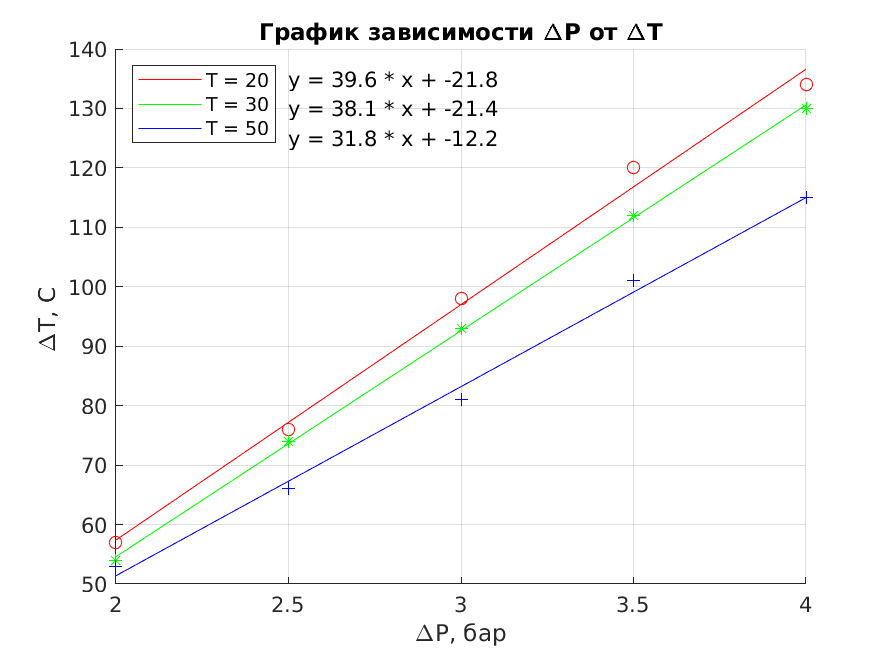
\includegraphics[width=15cm]{graph.png}
}







 













 




\end{document}